%\input{head.tex}
\subsection{Graphene and hydrogen honeycomb lattice}
Although only the low energy degrees of freedom are present in the downfolded Hamiltonian, the coefficients of various interacting terms are affected by the high energy degrees of freedom. In other words, the coefficients are renormalized by the high energy degrees of freedom. We demonstrate this renormalization effects from higher energy degree of freedom with two \textit{ab initio} honeycomb lattice  systems, graphene and hydrogen. 

Although many electronic properties of graphene can be correctly described in a noninteracting tight-binding model of $\pi$ electrons~\cite{Castro2009}, electron-electron interactions do play a central role in a wide range of phenomena that have been observed in experiments~\cite{Kotov2012}. It is shown that the electron screening from $\sigma$ bonding is very crucial to the correlated physics of graphene. \cite{Zheng2016}. The screening from $\sigma$ electrons renormalizes the low energy plasmon frequency of $\pi$ electrons~\cite{Zheng2016}. Without taking into effect of the $\sigma$ electrons, a system of $\pi$ electrons with bare Coulomb interaction is an insulator instead of a semimetal~\cite{DrutPRL2009, DrutPRB2009,  Smith2014, Zheng2016}. Therefore, studying the effect of $\sigma$ electrons on the low energy effective model of graphene. This provides an alternative perspective to understand the $\sigma$ screening effect. 

In order to disentangle the screening effect of $\sigma$ electrons from the bare interaction between $\pi$ electrons, we also consider a $\pi$-only graphene, in which the $\sigma$ electrons are replaced with a static constant negative charge background. The effect of $\sigma$ electrons could then be understood by comparing the effective model of these two systems. 
We here also study the hydrogen honeycomb lattice as a comparison. It is shown that the hydrogen system (with the same lattice constant $a=2.46$\AA~as graphene) has similar Dirac cone dispersion as graphene~\cite{Zheng2016}. We expect that the single body term should be similar to graphene. However, because of the difference in high energy orbitals, the electron-electrons interaction terms are expected to be different between graphene and hydrogen. 

The low energy physics is reflected mainly on the dynamics of $\pi$ orbitals in graphene, and $s$ orbitals in hydrogen (see Fig.~\ref{fig:honeycomb_wan}). We therefore consider the following We consider the effective single-band Hubbard model of $\pi$ orbitals (or $s$ orbitals in hydrogen) for the three systems, 
\begin{eqnarray}\label{eq:hubbard}
\hat{H} = C + t\sum_{\langle i,j\rangle}c_{i, \sigma}^\dagger c_{j, \sigma} + \text{h.c.} + U\sum_{i}n_{i, \uparrow}n_{i, \downarrow}\,. 
\end{eqnarray}
Due to the lack of screening because of the zero density of states at Fermi level, the Coulomb interaction is still long range unlike the case in metal where the Coulomb interaction is short ranged because of the formation of electron-hole pairs \cite{Zheng2016}. 
However, the effect of the long range part can be considered as a renormalization to the onsite Coulomb interaction $U$ at low energy \cite{Schuler2013, Changlani2015}. 
Therefore, we expect that Eq.~\eqref{eq:hubbard} is still a relatively good description of the low energy physics. 
\begin{figure}[hbt]
  \centering  
 % \subfigure[]{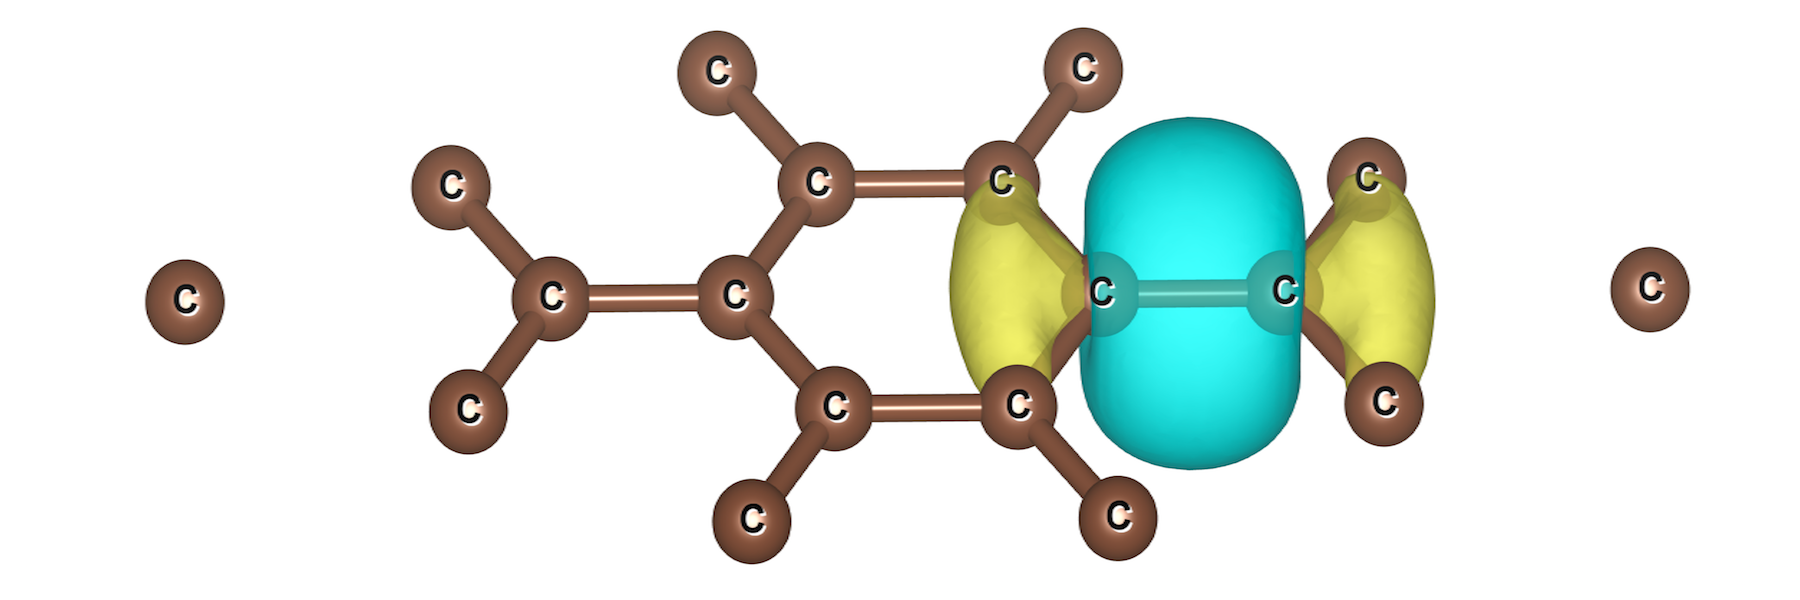
\includegraphics[clip, width=0.30\textwidth]{c_sigma.png}}
    \subfigure[]{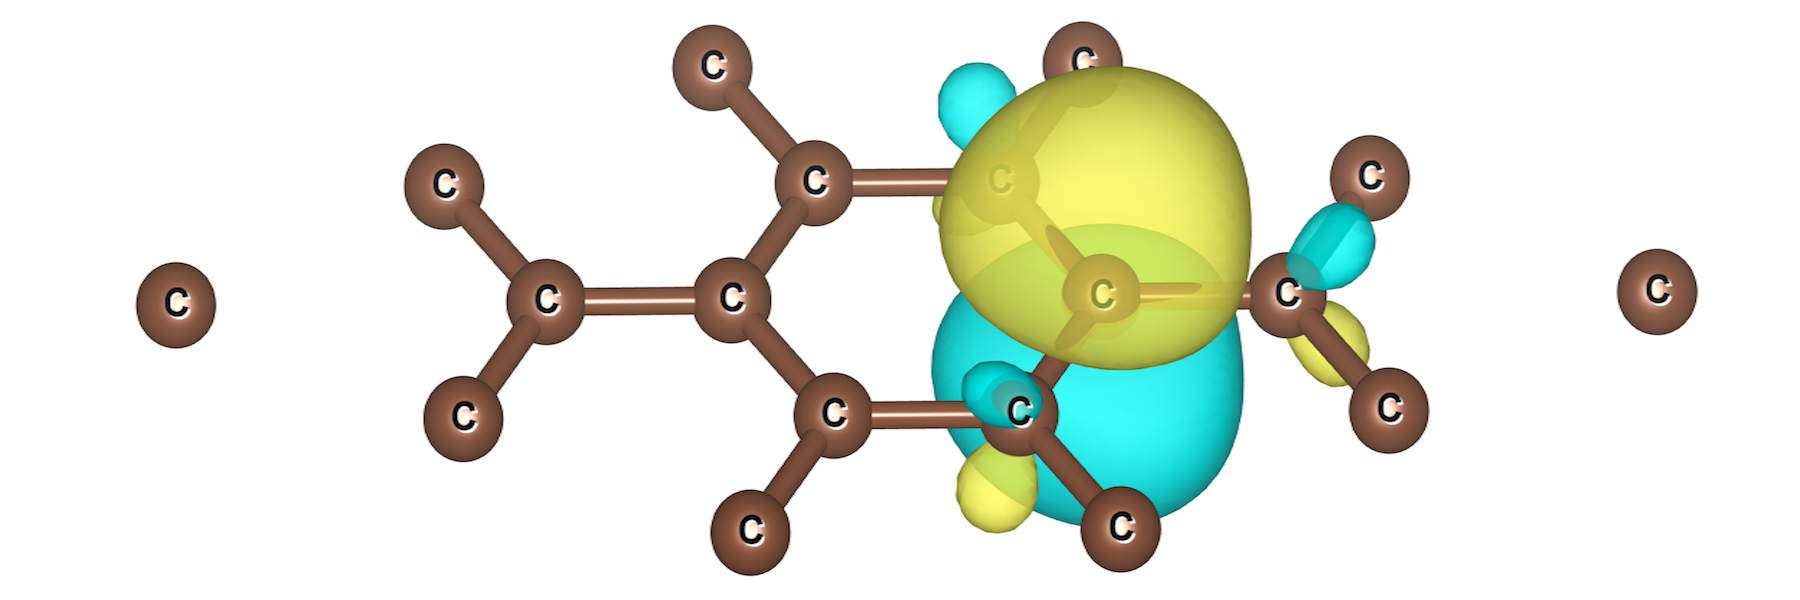
\includegraphics[clip, width=0.45\textwidth]{./Figures/c_pi.png}}
    \subfigure[]{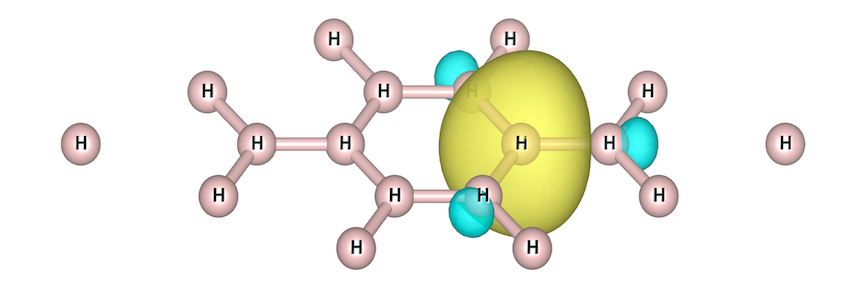
\includegraphics[clip, width=0.45\textwidth]{./Figures/h_wan.png}}
       \caption{Wannier orbitals constructed from Kohn-Sham orbitals: (a) graphene $\pi$ orbitals; (b) hydrogen S orbital. }
\label{fig:honeycomb_wan}
\end{figure}

We used the non-eigenstate AIDMD method for downfolding. We chose a set of Slater-Jastrow wave functions corresponding to the electron-hole excitations within the $\pi$ channel (or $s$ channel for hydrogen system). In particular, for graphene, the Slater-Jastrow wave functions are constructed from occupied $\sigma$ bands and occupied $\pi$ bands, whereas for $\pi$-only graphene, Slater-Jastrow wave functions constructed from occupied $\pi$ Kohn-Sham orbitals of graphene. The \textit{ab initio} simulations are performed on a $3\times3$ cell with the energy and reduce density matrices evaluated with variational Monte Carlo (VMC). We have used using $50$ low energy states for the downfolding. The error-bar is calculated using Jackniff method. 
%%%%% I omit the following equation and expect other section to provide detailed instruction on the methodology.
%The energy expectation expressed in terms of the density matrices is, 
%\begin{eqnarray}\label{eq:en}
%E = C + t\sum_{\langle i, j\rangle, \sigma}( \rho_{ij}^\sigma + \rho_{ji}^\sigma) + U \sum_{i}M_{ii;ii}^{\uparrow,\downarrow}\,.
%\end{eqnarray}
%where $\rho$ and $M$ are one- and two-body reduce density matrices respectively.


Table~\ref{tab:grpheffm} shows the final downfolding results of the three systems, and Fig.~\ref{fig:ne_aidmd_gh} shows the quality of the downfolding for the three systems.
\begin{table}[ht]
\label{tab:grpheffm}
\centering
\begin{tabular}{|c|c|c|c|}
\hline
Parameters [eV] & graphene & $\pi$-only graphene &hydrogen \\
\hline
\hline
t & 3.61(1) & 2.99(1) & 3.73(1)\\
U & 7.16(3) & 14.8(2) & 9.47(5)\\
\hline
\end{tabular}
\caption{Downfolding parameters for graphene and hydrogen.}
\end{table} 
We find that the onsite Hubbard model describes graphene and hydrogen very well, as is seen from the small root mean square error of the predicted energies (see Fig.~\ref{fig:ne_aidmd_gh}). The ratio of $U/t$ is small than the semi-metal-insulator transition critical value (3.8) in both graphene and hydrogen, which is consistent to the fact that both the two systems are semimetals. These two systems indeed has similar hopping constant $t$, consistent to the fact that they have similar Fermi velocity at Dirac point. They have different $U$ due to different high energy degrees of freedom. 

The $\pi$-only graphene has larger $U/t$ compared with graphene, and is in the insulating phase. On one hand, graphene has larger magnitude of $t$ than $\pi$-only graphene. This is because the $\sigma$ electrons push $\pi$ electrons away from the ions through exchange-correlation interaction, and $\pi$ electrons easier to hop to nearby sites. On the other hand, graphene has smaller $U$. 
This clearly shows the significance of $\sigma$ electrons in renormalizing the effective onsite interactions of $\pi$ orbitals. Therefore, the presence of $\sigma$ electrons changes both $t$ and $U$, and making graphene a weakly interacting semimetal. Without $\sigma$ electrons, graphene would be an insulator. This is consistent with previous studies which show that a system of $\pi$ electrons with bare Coulomb interaction is an insulator~\cite{DrutPRL2009, DrutPRB2009,  Smith2014}. 
\begin{figure*}[tbh]
\centering
  \begin{tabular}{@{}p{0.95\linewidth}@{\quad}p{\linewidth}@{}}
    \subfigimg[clip, width=0.32\linewidth]{(a)}{./Figures/grp_all_tu.pdf}
     \subfigimg[clip, width=0.32\linewidth]{(b)}{./Figures/grp_pi_tu.pdf}
    \subfigimg[clip, width=0.32\linewidth]{(c)}{./Figures/h_tu.pdf}
      \end{tabular}
\caption{Comparison of \textit{ab initio} (x-axis) and fitted energies (y-axis) of the 3$\times$3 periodic unit cell of graphene and hydrogen lattice: (a) graphene; (b) $\pi$-only graphene; (c) hydrogen lattice.}\label{fig:ne_aidmd_gh}
\end{figure*}

In summary, we have demonstrated that the effective models constructed using this approach effectively reflect the renormalization/screening effect from high energy degree of freedom, and correctly characterize the low energy dynamics of the system. 
%\input{tail.tex}
